\chapter{结构学习}
\label{chap:pgm-structure-learning}

已有的设备模型把故障、过热和报警连接成一张图，然后在这张图上估计参数、回答查询。如果手中只有运行记录，没有预先给定的连线，能否从数据中找出图？即使找到了稳定的连线，能否进一步断言箭头就是故障传播的方向？这两个问题看似相近，所需的信息却不同：数据可以支持某种依赖表示，而因果方向还取决于数据怎样产生，以及允许哪些替代解释。

第~\ref{chap:pgm-directed}章和第~\ref{chap:pgm-undirected}章说明了给定图如何约束分布，第~\ref{chap:pgm-parameter-learning}章则固定图来估计参数。本章把图也作为未知量。理解这一变化，需要把三个环节分开：条件独立检验提供局部证据，结构评分比较整个候选模型，搜索算法决定到哪里寻找候选。图的表示方式限制可搜索的对象，缺失和潜变量改变可利用的证据，因果假设决定所得结构能解释到哪一步。

\section{结构学习的定义}
\label{sec:pgm-structure-learning-definition}

设节点集合为$V=\{1,\ldots,d\}$，随机向量为$\bm{X}=(X_1,\ldots,X_d)^{\top}$，完整观测数据为$\mathcal{D}=\{\bm{x}_r:r=1,\ldots,n\}$。本章先假定这些样本独立同分布，缺失数据和多干预环境在相应小节另行说明。给定候选图族$\mathfrak{G}$及每张图对应的分布族$\mathcal{M}(\mathcal{G})$，\term{结构学习}（structure learning）就是利用数据和领域知识，选择或评价哪些图适合表示变量之间的依赖。候选图族不仅规定边的类型，也可以限定最大父集、禁止某些边，或者只允许树。

结构学习的输出不一定是一张完全定向的图。为了预测，可以选一个拟合与复杂度折中的有向图；为了表达不确定性，可以保留图上的后验分布；高斯模型可以输出稀疏精度矩阵；若数据只能区分一组图，就应输出这组图的共同信息。不同输出不是同一结果的绘图风格，而是对“哪些结论已被确定”的不同承诺。

对有向图，尤其需要理解这种承诺的限度。\term{Markov等价类}（Markov equivalence class, MEC）由具有相同d-分离关系的有向图组成。两张有向图属于同一等价类，当且仅当它们有相同的\term{骨架}（skeleton），即忽略方向后的邻接关系，以及相同的\term{无屏蔽碰撞结构}（unshielded collider，又称v-structure），即$i\to k\leftarrow j$且$i,j$不相邻。这里比较的是图蕴含的全部条件独立关系，不是某组参数碰巧产生的独立性。完整的等价性刻画可参见图模型教材\scite{pgm-koller2009}

在不附加函数形式限制的有向图模型中，等价图描述同一个分布族。三节点链$X_1\to X_2\to X_3$、反向链$X_1\leftarrow X_2\leftarrow X_3$和分叉$X_1\leftarrow X_2\to X_3$都只要求$X_1\perp X_3\mid X_2$；碰撞图$X_1\to X_2\leftarrow X_3$却要求两端边缘独立，因而不在这个等价类中。图~\ref{fig:pgm-structure-learning-equivalence}把“有三张图”与“只能确认什么”放在一起比较。

\begin{figure}[htbp]
  \centering
  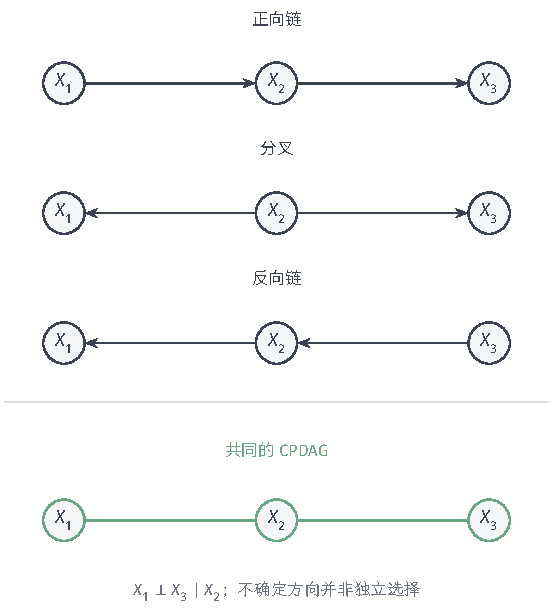
\includegraphics[width=\linewidth]{figures/03-models/03-probabilistic-graphical-models/tikz/pgm-structure-learning-equivalence/figure.pdf}
  \caption{三个无碰撞有向图共享骨架和条件独立关系，以底部的CPDAG统一表示。无向边表示方向在类内可变，不表示两个方向同时存在；把两条边同时指向$X_2$会产生新碰撞结构，不是合法补全。}
  \label{fig:pgm-structure-learning-equivalence}
\end{figure}

\term{完成的部分有向无环图}（completed partially directed acyclic graph, CPDAG）以一张部分定向图表示一个有向图等价类：类内所有有向图都具有的方向画为箭头，其余边画为无向边。它也称观测本质图。CPDAG中未定向边的选择相互约束，不能逐条任意定向；完成后的图必须无环，并且不增加新的无屏蔽碰撞结构。本文说“恢复CPDAG”，指恢复等价类的这些不变信息，而不是挑选一个代表后把其余方向也当作证据。

无向图没有方向选择，但仍有$2^{\binom d2}$种简单图。有向图除邻接外还需选择方向并排除有向环；仅固定一个拓扑序，就已有$2^{\binom d2}$种边集可选。含不同端点标记的混合图可以表达潜变量边缘化后的结构，其合法性也受到全局限制。因此，模型的表达能力、参数量和搜索代价必须一起考虑：较大的图族能容纳更多分布，却要求更多数据，也更难遍历。若还需频繁推断，树宽等计算性质可以成为明确的候选约束，但不能把这种工程约束说成从数据中发现的事实。

\section{有向图结构学习}
\label{sec:pgm-structure-learning-directed}

同一组数据既可以接受条件独立检验，也可以用于计算似然。前者把结构证据写成“给定哪些变量后可以删去联系”，后者把证据累积成候选图的分数。搜索可以只依靠一种证据，也可以组合二者；它不是与检验、评分并列的第三种统计假设。

\subsection{条件独立约束}
\label{sec:pgm-structure-learning-constraints}

为了从独立性反推边，需要假定分布中的条件独立恰好来自某张有向图的d-分离。这称为\term{忠实性}（faithfulness）：图上的d-连接不会因参数抵消而产生额外独立性。在这个假设下，找到了使$X_i$与$X_j$条件独立的集合$S\subseteq V\setminus\{i,j\}$，就有理由删去$i,j$之间的边。有限样本中未知的是条件分布，因此算法实际检验
\[
  H_0:X_i\perp X_j\mid\bm{X}_S,
\]
并把未拒绝$H_0$暂作删边依据。未拒绝不等于证明独立；如果检验没有足够功效，真实但较弱的联系也可能被删去。

有限离散变量可使用分层列联表。令$N_{a,b,s}$为$(X_i,X_j,\bm{X}_S)=(a,b,s)$的样本数，点号表示对相应指标求和。似然比检验统计量为
\begin{equation}
  G^2=2\sum_{a,b,s:N_{a,b,s}>0}
  N_{a,b,s}\log
  \frac{N_{a,b,s}N_{\cdot,\cdot,s}}
       {N_{a,\cdot,s}N_{\cdot,b,s}}.
  \label{eq:pgm-structure-learning-g-test}
\end{equation}
在各单元概率为正、样本足够且变量状态数固定时，它在原假设下渐近服从卡方分布；若条件变量共有$q_S$种配置，自由度为$q_S(r_i-1)(r_j-1)$，其中$r_i,r_j$为两端状态数。小样本、结构性零单元或许多稀有配置会破坏这项近似，不能只把自由度代入软件就认为检验可靠。

\term{条件互信息}（conditional mutual information）衡量给定条件后，联合分布偏离条件边缘乘积的程度。对有限离散变量，其定义为
\[
  I(X_i;X_j\mid\bm{X}_S)
  =\sum_{a,b,s}p(a,b,s)
       \log\frac{p(a,b\mid s)}{p(a\mid s)p(b\mid s)}.
\]
求和只计入正概率项；这一量是各条件配置下KL散度的加权平均，非负且恰在条件独立时为零。以经验频率代入就得到$\widehat I=G^2/(2n)$。$S$为空时，条件互信息退化为\term{互信息}（mutual information），衡量两端的边缘依赖；较大的互信息不一定表示存在一条直接边。

对联合高斯变量，条件独立等价于偏相关$\rho_{i,j\mid S}=0$。偏相关是分别用$\bm{X}_S$线性回归两端以后，两个残差的相关系数；这给出了直接的计算办法。样本偏相关$\widehat\rho$经Fisher变换得到
\[
  Z=\frac{\sqrt{n-|S|-3}}{2}
    \log\frac{1+\widehat\rho_{i,j\mid S}}
                  {1-\widehat\rho_{i,j\mid S}},
\]
在相应正则条件下近似服从标准正态分布。非高斯分布中，零偏相关通常不够；核条件独立检验可以考察更丰富的非线性关系，但核、正则化和零分布校准都会影响结论。也不能用一般回归残差“不相关”来代替原变量的条件独立。

为使后续比较可以复核，本章使用三个二值测量量$X_1,X_2,X_3$。它们可理解为同一设备的三项状态指示，但不沿用前章故障模型的参数。表~\ref{tab:pgm-structure-learning-counts}是专为计算构造的100条记录，不是真实测量结果。每个变量都恰有50个$0$和50个$1$。

\begin{table}[htbp]
  \centering
  \begin{tabular}{ccc r@{\qquad}ccc r}
    \toprule
    $x_1$ & $x_2$ & $x_3$ & 次数 & $x_1$ & $x_2$ & $x_3$ & 次数 \\
    \midrule
    0 & 0 & 0 & 36 & 1 & 0 & 0 & 4 \\
    0 & 0 & 1 & 9  & 1 & 0 & 1 & 1 \\
    0 & 1 & 0 & 1  & 1 & 1 & 0 & 9 \\
    0 & 1 & 1 & 4  & 1 & 1 & 1 & 36 \\
    \bottomrule
  \end{tabular}
  \caption{人工构造的二值数据。记录恰好匹配公平根变量经过两次独立翻转的分布，两次翻转概率分别为$0.1$和$0.2$。这只是生成数据的一种表示，不能由该表唯一确定因果方向。}
  \label{tab:pgm-structure-learning-counts}
\end{table}

将经验频率记为$\widehat p$。表中$\widehat p(X_1=1,X_3=1)=0.37\ne0.25$，两端有边缘依赖；但给定$X_2=0$时，
\[
  \widehat p(X_1=0,X_3=0\mid X_2=0)
  =\frac{36}{50}=\frac{45}{50}\frac{40}{50}.
\]
这一层的其余三格也满足乘积分解，$X_2=1$层同样如此。因此经验条件互信息为零，式~\eqref{eq:pgm-structure-learning-g-test}给出$G^2=0$。这是人为设计的精确等式；一般样本即使来自条件独立分布，也不会恰好满足它。

\term{PC算法}（PC algorithm）把这类局部检验组织成结构恢复过程。它从完全无向图出发，按$|S|=0,1,\ldots$增加条件集大小；对尚相邻的$i,j$，从$i$的当前邻接集合去掉$j$后选取$S$，也考察交换两端后的候选。一旦未拒绝条件独立，就删边并记录一个分离集$\operatorname{Sep}(i,j)$。当所有相邻点对都没有足够大的候选邻接集合时，骨架阶段停止。在忠实性及准确独立性判定下，这种邻域搜索足以找到所需分离集，避免枚举所有节点子集。

骨架确定以后，对每个无屏蔽三元组$i-k-j$，若$k\notin\operatorname{Sep}(i,j)$，就将其定向为$i\to k\leftarrow j$。随后反复应用保持等价类的定向规则。例如，已有$i\to k-j$且$i,j$不相邻时，$k-j$必须成为$k\to j$，否则会引入一个此前未确认的碰撞；已有$i$到$j$的有向路径时，边$i-j$不能定为$j\to i$，否则形成有向环。完整实现需要完整的定向规则集，不是只执行这两个示意规则；在总体判定正确时，最终得到CPDAG。PC的高维高斯一致性分析明确依赖稀疏性及非零偏相关不能过小等条件\scite{pgm-structure-learning-kalisch2007}

对表~\ref{tab:pgm-structure-learning-counts}，三对变量的边缘检验统计量为
\[
  \begin{aligned}
    G^2_{1,2}&\approx73.6128,\\
    G^2_{2,3}&\approx38.5490,\\
    G^2_{1,3}&\approx24.0181.
  \end{aligned}
\]
若用显著性水平$0.05$的渐近检验演示流程，它们都超过自由度为1时的临界值$3.841$。给定$X_2$后，两端的条件检验统计量为零，于是删除$1-3$边，记录分离集$\operatorname{Sep}(1,3)=\{2\}$。结果为$1-2-3$，没有证据选择图~\ref{fig:pgm-structure-learning-equivalence}中的某一个方向。此例条件表含稀有格，仅用于展示流程，不据此保证小样本卡方校准准确。

若一次检验误把$1,3$判为边缘独立，记录的分离集会变为空集，接着就可能错误地定向为碰撞结构。误删边还会缩小后续可搜索的邻接集合，改变后面的检验和定向。有限样本实现须记录冲突处理与节点处理顺序，必要时采用稳定化的邻接更新，而不能假定所有检验决定总能组成合法CPDAG。

\subsection{结构评分与后验}
\label{sec:pgm-structure-learning-scores}

条件独立检验一次回答一个问题，评分则问一张图对全部数据的解释是否值得其复杂度。在观测完整且模型不含潜变量的离散设定下，设$X_i$有$r_i$个状态，其父集共有$q_i$种配置。令$N_{i,j,k}$统计节点$i$取第$k$个状态且父集取第$j$种配置的次数，$N_{i,j}=\sum_kN_{i,j,k}$。在各条件概率表自由变化时，最大似然对数得分为
\begin{equation}
  \ell(\widehat{\bm{\theta}}_{\mathcal{G}};\mathcal{D})
  =\sum_{i=1}^{d}\sum_{j=1}^{q_i}\sum_{k=1}^{r_i}
    N_{i,j,k}\log\frac{N_{i,j,k}}{N_{i,j}}.
  \label{eq:pgm-structure-learning-local-likelihood}
\end{equation}
零计数项按$0\log0=0$处理；若一整行未出现，该行条件分布不由数据决定，不能真的计算$0/0$。对数似然按节点分解，所以改动一个父集只改变相应局部项。

但未惩罚似然会奖励多余边。若$\mathcal{M}(\mathcal{G}_1)\subseteq\mathcal{M}(\mathcal{G}_2)$，最大化后必有$\ell_2\geq\ell_1$；更大的模型至少可以把新增依赖的参数设成无作用。因此，未惩罚最大似然适合在复杂度已固定的模型之间比较，一般结构选择还需要复杂度控制。\term{贝叶斯信息准则}（Bayesian information criterion, BIC）在本章采用越大越好的记号：
\begin{equation}
  \begin{aligned}
    \operatorname{Score}_{\mathrm{BIC}}(\mathcal{G})
      &=\ell(\widehat{\bm{\theta}}_{\mathcal{G}};\mathcal{D})
        -\frac{k_{\mathcal{G}}}{2}\log n,\\
    k_{\mathcal{G}}&=\sum_iq_i(r_i-1).
  \end{aligned}
  \label{eq:pgm-structure-learning-bic}
\end{equation}
常见软件把它乘以$-2$并最小化，二者排序相同。这里$k_{\mathcal{G}}$是自由参数数目，不是边数。BIC作为对数边缘似然的渐近近似，需要固定维数、内部参数和非奇异信息矩阵等正则条件；潜变量模型往往不满足这些条件。

\term{最小描述长度}（minimum description length, MDL）从编码角度作同样的权衡：用多少信息描述模型，又用多少信息描述模型没有预测好的数据。某些MDL近似产生与BIC相同的主导惩罚，但具体编码还可能包含图结构的码长，不应把所有MDL评分都写成唯一的BIC公式。无论选哪种准则，都须固定参数化、复杂度定义及得分方向后再进行搜索。

表~\ref{tab:pgm-structure-learning-counts}中，独立模型有3个参数，任一无碰撞链有5个，完整三节点有向图有7个。以自然对数计算，三者的最大对数似然分别为$-207.9442$、$-151.8633$、$-151.8633$。完整图虽然能表示更多分布，对这张特制的表却没有额外拟合收益。对应BIC为$-214.8519$、$-163.3762$、$-167.9814$，所以链优于完整图。这个比较选择了依赖复杂度，却仍没有区分三种等价方向。

另一种办法不先把参数优化为一点，而是把它积分掉。\term{边缘似然}（marginal likelihood）是参数先验下的平均数据似然，结构后验据此写成
\begin{equation}
  \begin{aligned}
    p(\mathcal{D}\mid\mathcal{G})
      &=\int p(\mathcal{D}\mid\bm{\theta},\mathcal{G})
              p(\bm{\theta}\mid\mathcal{G})\,\mathrm{d}\bm{\theta},\\
    p(\mathcal{G}\mid\mathcal{D})
      &\propto p(\mathcal{D}\mid\mathcal{G})p(\mathcal{G}).
  \end{aligned}
  \label{eq:pgm-structure-learning-posterior}
\end{equation}
它奖励能在先验支持的较大参数区域内解释数据的结构，而不是只奖励某个极窄区域内的最佳拟合；这种复杂度控制也意味着先验不可忽略。

比较两个候选结构时，\term{Bayes因子}（Bayes factor）是它们的边缘似然之比，衡量数据使两者的相对支持改变了多少。设模型内参数先验均已归一化，两个边缘似然有限，且第二个严格为正，则
\begin{equation}
  \begin{aligned}
    \operatorname{BF}_{12}
      &=\frac{p(\mathcal{D}\mid\mathcal{G}_1)}
              {p(\mathcal{D}\mid\mathcal{G}_2)},\\
    \frac{p(\mathcal{G}_1\mid\mathcal{D})}
         {p(\mathcal{G}_2\mid\mathcal{D})}
      &=\operatorname{BF}_{12}
        \frac{p(\mathcal{G}_1)}{p(\mathcal{G}_2)}.
  \end{aligned}
  \label{eq:pgm-structure-learning-bayes-factor}
\end{equation}
第二式还要求结构先验$p(\mathcal{G}_2)>0$，且全体候选结构给出的数据证据有限而为正。左侧是后验赔率，右侧将它分成数据贡献与结构先验赔率。Bayes因子依赖各结构内部的参数先验，却不包含外层结构先验赔率。例如$\operatorname{BF}_{12}=3$而先验赔率为$1/2$时，后验赔率为$3/2$，不是$3$。

仍在观测完整且模型不含潜变量的离散设定下，若各条件表行参数$\bm{\theta}_{i,j}$在先验下独立，并采用狄利克雷先验$\bm{\theta}_{i,j}\sim\operatorname{Dir}(\alpha_{i,j,1},\ldots,\alpha_{i,j,r_i})$，其中$\alpha_{i,j,k}>0$且$\alpha_{i,j}=\sum_k\alpha_{i,j,k}$，积分可精确计算。每行似然与先验相乘后，$\theta_{i,j,k}$的指数从$\alpha_{i,j,k}-1$变成$\alpha_{i,j,k}+N_{i,j,k}-1$，所以积分就是更新前后狄利克雷归一化常数之比。各行相乘得到
\begin{equation}
  p(\mathcal{D}\mid\mathcal{G})
  =\prod_{i,j}
    \frac{\Gamma(\alpha_{i,j})}
         {\Gamma(\alpha_{i,j}+N_{i,j})}
    \prod_k
    \frac{\Gamma(\alpha_{i,j,k}+N_{i,j,k})}
         {\Gamma(\alpha_{i,j,k})}.
  \label{eq:pgm-structure-learning-dirichlet}
\end{equation}
这里$\mathcal{D}$是逐条记录的样本，故没有另乘一个依结构改变的多项式计数系数。任意指定各行狄利克雷超参数都可得到这类贝叶斯狄利克雷评分，但不一定具有评分等价性。

\term{贝叶斯狄利克雷等价评分}（Bayesian Dirichlet equivalent score, BDe）要求等价有向图取得相同边缘似然。实现它的一种方式是给出一个严格为正的先验联合分布$p_0$和共同的\term{等效样本量}（equivalent sample size）$\alpha>0$，按每个候选父集的边缘概率设置
\[
  \alpha_{i,j,k}
  =\alpha\,p_0(X_i=k,\bm{X}_{\operatorname{pa}(i)}=j).
\]
式中的$j,k$在这里代表相应配置的编号。这些伪计数来自同一个联合分布，而不是在每张图上互不协调地指定。结合参数独立性、参数模块性和似然等价性假设，可得到等价图相同的积分；若结构先验$p(\mathcal{G})$在类内不同，结构后验仍可不同，不能把先验造成的偏好归因于数据\scite{pgm-structure-learning-heckerman1995}

\term{均匀BDe评分}（BDe uniform, BDeu）取均匀$p_0$，于是$\alpha_{i,j,k}=\alpha/(q_i r_i)$。这是BDe的特例，不意味着每张图的结构先验均匀，也不意味着每个条件表行有相同的总伪样本量$\alpha$；每行实际只有$\alpha/q_i$。例如二值$X_2$有一个二值父节点且$\alpha=4$时，每格伪计数为1。表中的父状态$X_1=0$对应$(45,5)$次观测，后验均值为$(46/52,6/52)$，而不是最大似然估计的$(0.9,0.1)$。增加父节点会增加$q_i$，把同一总量分散到更多配置；数据稀疏时，不同$\alpha$可能显著改变结构排序，应报告敏感性。

仍取$\alpha=4$，将表~\ref{tab:pgm-structure-learning-counts}的计数代入式~\eqref{eq:pgm-structure-learning-dirichlet}，正向链、分叉和反向链的对数边缘似然均约为$-161.968668$。这一数值既可复核公式，也说明BDeu不会仅因把同一个无碰撞链改画成另一方向就奖励其中一张图。

如果多张图都能解释数据，单一最优图会掩盖这种不确定性。\term{贝叶斯模型平均}（Bayesian model averaging, BMA）按结构后验综合预测：
\[
  p(\bm{x}_{\mathrm{new}}\mid\mathcal{D})
  =\sum_{\mathcal{G}\in\mathfrak{G}}
    p(\bm{x}_{\mathrm{new}}\mid\mathcal{D},\mathcal{G})
    p(\mathcal{G}\mid\mathcal{D}).
\]
每项预测还需积分参数后验。对“存在某条边”这样的结构特征，也可把其指示函数按同一后验加权。实际计算常用结构采样或一组高分候选近似，必须说明只覆盖了哪些图；搜索多次得到同一图不等于已计算其后验概率。对等价类平均时还要明确先验作用于有向图还是等价类，不能把类内图的数量差异悄悄忽略。

\subsection{结构空间搜索}
\label{sec:pgm-structure-learning-search}

定义了评分，还没有解决怎样找到高分图。有向图局部搜索从一张满足约束的图开始，尝试加边、删边、反向三种操作；每个候选都要检查无环性和领域限制，然后接受得分最大的正增益操作。当没有合法改进时停止，所得只是该邻域中的局部最优。加边只需更新一个局部评分，反向需更新两端评分；缓存父集得分可以减少重复计算，但不能消除全局无环约束。重启、禁忌搜索或更大邻域可以探索更多位置，不提供无条件的全局最优保证。

离散BIC还能把一次加边的得分变化写得很清楚。设向$X_i$的现有父集$P$加入$X_j$，用$\widehat I$表示经验条件互信息，则
\begin{equation}
  \Delta\operatorname{Score}_{\mathrm{BIC}}
  =n\widehat I(X_i;X_j\mid\bm{X}_P)
   -\frac{\Delta k}{2}\log n.
  \label{eq:pgm-structure-learning-score-gain}
\end{equation}
第一项来自条件熵的减少，第二项是新增自由参数的代价。表中从空图加入$1\to2$时，$\widehat I(X_1;X_2)=0.368064$，$\Delta k=1$，增益为$36.8064-2.3026=34.5038$。互信息在这里进入评分，并不意味着算法正在执行固定显著性水平的独立性检验。已经确定的评分和执行移动的搜索仍是两个环节。

评分等价时，有向图搜索会反复走过得分相同的代表。\term{贪心等价搜索}（greedy equivalence search, GES）把状态改为CPDAG，在等价类之间先做前向插入，再做后向删除，各阶段都在没有正增益合法操作时停止。一次等价类操作可能同时规定若干端点方向，再完成为新的CPDAG，不能简单理解为在当前画面上任意添一条箭头。GES的理论保证依赖评分等价、局部一致性及真实分布存在有向图完美映射等条件，并不说明任何局部爬山法都能成功\scite{pgm-structure-learning-chickering2002}

当节点数允许时，也可以作精确搜索。对可分解评分，记$s_i(P)$为节点$i$选择父集$P$的得分，$F(U)$为节点子集$U$上最佳有向图得分。任一非空有向图都有一个汇点，即没有出边的节点，所以
\begin{equation}
  \begin{aligned}
    F(\varnothing)&=0,\\
    F(U)&=\max_{i\in U}\left\{
      F(U\setminus\{i\})
      +\max_{P\subseteq U\setminus\{i\}}s_i(P)\right\}.
  \end{aligned}
  \label{eq:pgm-structure-learning-dp}
\end{equation}
递推把$i$放在拓扑序末尾，剩余图与$i$的父集即可独立优化；枚举所有可能汇点就覆盖全部有向图。预计算最佳父集得分后，这类动态规划仍需处理指数多的子集，精确性是用时间和内存换来的。

整数规划则为每个候选父集设置二值变量$z_{i,P}$，以$\sum_{i,P}s_i(P)z_{i,P}$为目标，并要求$\sum_Pz_{i,P}=1$。还必须阻止所选父集组成环。例如对每个非空$U\subseteq V$要求
\[
  \sum_{i\in U}\ \sum_{P:P\cap U=\varnothing}z_{i,P}\geq1.
\]
它要求每个诱导子图至少有一个在子图内无父节点的点；有向环的节点集合不满足这一条件，而有向图总满足。约束数量指数增长，求解器通常按需加入违反的约束。只有完成最优性认证，才可说得到所规定候选空间内的最优解；提前截断的父集空间同样限制结论。

连续优化改变的是搜索表示。令$\bm{W}\in\mathbb{R}^{d\times d}$满足$W_{i,j}\ne0$对应$i\to j$，$\bm{Y}\in\mathbb{R}^{n\times d}$为中心化数据矩阵，每行是一条样本。NOTEARS把线性模型的拟合写成
\begin{equation}
  \begin{aligned}
    \min_{\bm{W}}\quad&
      \frac{1}{2n}\lVert\bm{Y}-\bm{Y}\bm{W}\rVert_{\mathrm F}^{2}
      +\lambda\lVert\bm{W}\rVert_1,\\
    \text{满足}\quad&
      h(\bm{W})=
      \operatorname{tr}\!\left(\exp(\bm{W}\circ\bm{W})\right)-d=0.
  \end{aligned}
  \label{eq:pgm-structure-learning-notears}
\end{equation}
这里$\circ$为逐元素乘积，$\exp$是矩阵指数，不是逐元素指数；$\lVert\bm{W}\rVert_1$表示所有元素绝对值之和。令$\bm{B}=\bm{W}\circ\bm{W}$，则
\[
  h(\bm{W})=\sum_{m=1}^{\infty}
     \frac{\operatorname{tr}(\bm{B}^m)}{m!}.
\]
$\bm{B}$非负，而$\operatorname{tr}(\bm{B}^m)$累加长度为$m$的闭合有向游走的权重。有向环存在时，至少某一项严格为正；无环时所有闭合游走都不存在，每项为零。这证明$h(\bm{W})=0$与支撑图无环精确等价，也排除了自环。梯度为$2\bm{W}\circ[\exp(\bm{W}\circ\bm{W})]^{\top}$，可交给增广拉格朗日等数值方法\scite{pgm-structure-learning-zheng2018}

可微不等于凸：无环可行集合仍然非凸，数值求解也不保证全局最优。停止容差下的$h$接近零不意味着阈值化后的图必然无环，须另作拓扑检查。平方损失采用线性拟合尺度，其统计识别性质还依赖噪声和模型假设；无环公式本身既不要求非高斯，也不赋予所选方向因果真实性。

混合方法可以先用条件独立信息筛选候选邻接或父集，再在缩小后的空间内优化BIC、BDe等评分。这样做减少搜索量，也把筛选阶段的漏边变成后续无法修复的限制。因而“使用PC式筛选、BIC评分、有向图爬山搜索”是一套可组合的设计，不能把这些名字列成互斥模型类别。

\subsection{观测缺失与结构EM}
\label{sec:pgm-structure-learning-structural-em}

如果某些记录没有测量$X_2$，前面评分公式所需的$N_{i,j,k}$就无法直接计数。此时观测似然对每条记录先边缘化未观测变量，不再按节点简单分解。删去不完整记录还可能改变样本分布。下文假定缺失机制可忽略，例如满足随机缺失并且缺失机制参数与模型参数可区分；若缺失取决于未观测值，通常必须把缺失指示机制也纳入模型。

\term{结构期望最大化}（structural expectation maximization，结构EM）在当前图下推断缺失值，再利用这些推断结果比较新图。与固定图的EM不同，M步允许改变父集。以下以有限离散缺失变量为例，记所有未观测量为$\bm{Z}$，观测记录为$\mathcal{D}_{\mathrm{obs}}$，当前后验为
\[
  q^{(t)}(\bm{Z})
  =p(\bm{Z}\mid\mathcal{D}_{\mathrm{obs}},
                  \mathcal{G}^{(t)},\bm{\theta}^{(t)}).
\]
对某个候选图的节点家庭，所需期望计数是
\[
  \overline N_{i,j,k}^{(t)}
  =\sum_{r=1}^{n}
    \mathbb{E}_{q^{(t)}}\!
      \left[\mathbf{1}\{X_{r,i}=k,
        \bm{X}_{r,\operatorname{pa}_{\mathcal{G}}(i)}=j\}\right].
\]
$X_{r,i}$表示第$r$条记录中的节点$i$；已观测分量在期望中固定。候选图改变后，所需联合后验作用域也可能改变，因此E步不能只计算当前图已有边的边缘统计。

对惩罚似然版本，在相同未观测变量空间上定义
\begin{equation}
  \begin{aligned}
    Q^{(t)}(\mathcal{G},\bm{\theta})
      &=\mathbb{E}_{q^{(t)}}[
          \log p(\mathcal{D}_{\mathrm{obs}},\bm{Z}
                     \mid\mathcal{G},\bm{\theta})],\\
    \mathcal{F}^{(t)}(\mathcal{G},\bm{\theta})
      &=Q^{(t)}(\mathcal{G},\bm{\theta})+H(q^{(t)})
        -\operatorname{pen}(\mathcal{G}).
  \end{aligned}
  \label{eq:pgm-structure-learning-sem-bound}
\end{equation}
其中$H(q^{(t)})$是缺失值后验的熵，在本轮比较中固定。由Jensen不等式，$\mathcal{F}^{(t)}$是观测对数似然减惩罚的下界；当$q^{(t)}$为精确当前后验时，下界在当前模型处相切。记第$t$轮模型的观测对数似然减惩罚为$L^{(t)}$。只要搜索找到使$Q^{(t)}-\operatorname{pen}$不下降的新图及参数，就有
\[
  \begin{aligned}
    L^{(t+1)}
    &\geq \mathcal{F}^{(t)}(\mathcal{G}^{(t+1)},\bm{\theta}^{(t+1)})\\
    &\geq \mathcal{F}^{(t)}(\mathcal{G}^{(t)},\bm{\theta}^{(t)})
     =L^{(t)}.
  \end{aligned}
\]
完全数据对数似然对计数线性，所以此处用$\overline N^{(t)}$替换计数能够精确构造$Q^{(t)}$。这项单调性来自共同下界，不是因为新图的补全数据似然看起来更大。

例如，一条记录只观测到$X_1=X_3=0$，当前模型取表~\ref{tab:pgm-structure-learning-counts}对应的链参数。$X_2=0$和$1$的未归一化概率分别为$0.5\times0.9\times0.8=0.36$及$0.5\times0.1\times0.2=0.01$，故后验为$(36/37,1/37)$。这条记录给相应家庭计数贡献分数，而不是把缺失值硬填成$0$。若当前结构错了，这些软计数也可能持续偏向错误解释，结构EM仍可能停在局部解。

贝叶斯结构EM还涉及参数积分。对固定且可比较的未观测变量空间，精确贝叶斯版本用当前模型下已积分参数的未观测量后验，对候选的完全数据对数边缘似然取期望，再加入结构先验。式~\eqref{eq:pgm-structure-learning-dirichlet}含有非线性的$\log\Gamma$，一般有
\[
  \mathbb{E}[\log\Gamma(\alpha+N)]
  \ne\log\Gamma(\alpha+\mathbb{E}[N]).
\]
因此，把期望计数直接代入BDe只是近似，不是精确观测边缘似然，也不能直接继承精确贝叶斯结构EM的单调性。Friedman分别给出了贝叶斯结构EM的理论框架及实际计算所需近似\scite{pgm-structure-learning-friedman1998}

近似E步同样需要区分目标：变分E步可以改善自身下界，但未必提高真实观测似然；采样误差也可能导致错误接受结构。增加潜变量或改变潜在状态数会改变隐空间，不能不经处理沿用上面的相切下界证明。实践中常固定一组候选潜变量再优化，或者对新增候选单独初始化、拟合和比较。潜变量的标签置换、观测等价和其他不可识别性不会因重复E步消失。

\section{无向图结构学习}
\label{sec:pgm-structure-learning-undirected}

无向图的学习目标是条件依赖，不必解决箭头方向。困难仍取决于允许哪种分布和相互作用：树的分解产生一个组合优化特例，高斯分布把结构映射为矩阵的零元素，一般离散模型则要同时处理特征选择和归一化。

\subsection{树结构与Chow--Liu算法}
\label{sec:pgm-structure-learning-chow-liu}

对有限离散变量，若只允许树上的成对因子，每个候选树都只保留$d-1$条边。将树任选一个根并向外定向，它没有碰撞点，因而既可写成无向树分解，也可写成每个非根节点只有一个父节点的有向图。选择这个根只是计算表示，不是因果定向。

设$\mathcal{T}=(V,E_{\mathcal{T}})$是一棵生成树，经验单点边缘为$\widehat p_i$，成对边缘为$\widehat p_{i,j}$。只要每个声明状态的经验单点概率严格为正，固定树的最大似然分布就可写为
\begin{equation}
  \widehat p_{\mathcal{T}}(\bm{x})
  =\prod_{i=1}^{d}\widehat p_i(x_i)
   \prod_{\{i,j\}\in E_{\mathcal{T}}}
     \frac{\widehat p_{i,j}(x_i,x_j)}
          {\widehat p_i(x_i)\widehat p_j(x_j)}.
  \label{eq:pgm-structure-learning-tree-factor}
\end{equation}
边因子修正了独立模型遗漏的成对关系。与一般图上的成对因子不同，这个表达式已经归一化，不需要另求配分函数；原因就在于树可以从叶子逐个消去。

\begin{theorem}[Chow--Liu最优树]
  \label{thm:pgm-structure-learning-chow-liu}
  设$V=\{1,\ldots,d\}$为有限节点集合，每个$X_i$取值于有限非空状态空间，数据由$n\geq1$条完整记录组成。假定每个声明状态$a$均有$\widehat p_i(a)>0$；成对经验边缘允许取零。候选模型类由$V$上的全部生成树及其不受额外参数约束的局部概率表组成。定义自然对数下的经验互信息
  \[
    \widehat I(X_i;X_j)
    =\sum_{a,b}\widehat p_{i,j}(a,b)
       \log\frac{\widehat p_{i,j}(a,b)}
                     {\widehat p_i(a)\widehat p_j(b)}.
  \]
  其中$\widehat p_{i,j}(a,b)=0$的项按$0\log 0=0$解释。
  以$\widehat I(X_i;X_j)$为边权，任一最大权生成树$\mathcal{T}^{*}$及式~\eqref{eq:pgm-structure-learning-tree-factor}给出的分布，构成树族内的全局最大似然解。
\end{theorem}

\begin{proof}
  固定树$\mathcal{T}$并选择根$o$，用$\pi(i)$表示非根节点$i$唯一的父节点。任一树分布可写为
  \[
    q_{\mathcal{T}}(\bm{x})
    =q_o(x_o)\prod_{i\ne o}q_i(x_i\mid x_{\pi(i)}).
  \]
  对数似然分解为根边缘和每条条件表行的对数似然。各行分别受“概率之和为1”约束，独立极大化得到$q_o=\widehat p_o$及$q_i=\widehat p_{i,\pi(i)}/\widehat p_{\pi(i)}$。单点边缘的严格正性保证分母非零；零频成对单元只会使相应条件概率为零，不影响归一化或最优性。这些都是归一化的条件概率，由叶到根求和可知乘积也是归一化分布。将其整理，便得到式~\eqref{eq:pgm-structure-learning-tree-factor}；这同时证明了固定树上参数解的最优性。

  记$\widehat H(X_i)=-\sum_a\widehat p_i(a)\log\widehat p_i(a)$。将上述分布代入经验平均对数似然，并按单点和边的作用域求和，得到
  \begin{equation}
    \begin{aligned}
      \frac1n\ell(\widehat p_{\mathcal{T}};\mathcal{D})
      &=\mathbb{E}_{\widehat p}
          [\log\widehat p_{\mathcal{T}}(\bm{X})]\\
      &=-\sum_i\widehat H(X_i)
        +\sum_{\{i,j\}\in E_{\mathcal{T}}}
           \widehat I(X_i;X_j).
    \end{aligned}
    \label{eq:pgm-structure-learning-tree-score}
  \end{equation}
  熵项与树无关，所以树族中的最优结构正是互信息边权和最大的生成树。每个候选树的最佳参数都已包含在比较中，故这不是仅在某组固定参数下的结构最优。

  最大权生成树可用按权重递减加边的Kruskal算法得到，加入边时跳过会形成环的选择，同权边可按固定节点顺序处理。其最优性可由交换论证说明：设已选森林包含在某棵最优树中，新选边$e$连接森林的两个分量。若最优树不含$e$，把$e$加入会形成环；环上必有另一条边$f$跨过相应分量边界且不在当前森林中。$f$在本轮也是可选边，故$w(e)\geq w(f)$。以$e$替换$f$不会降低总权重，仍得到包含新森林的最优树。归纳到选满$d-1$条边，算法输出即为最优树。
\end{proof}

也可以从分布逼近看这个结果：$\operatorname{KL}(\widehat p\Vert\widehat p_{\mathcal{T}})$等于式~\eqref{eq:pgm-structure-learning-tree-score}右侧的负值再减去$\widehat H(\bm{X})$，后者同样不依赖树。因此，最大似然树也是对经验分布的最小KL树近似。把经验边缘换成给定总体分布的边缘，同一证明给出总体版本。这一经典结果由Chow与Liu提出\scite{pgm-structure-learning-chow1968}

表~\ref{tab:pgm-structure-learning-counts}的三个单点熵均为$\log2$。$X_1,X_2$不相等的频率为$0.1$，$X_2,X_3$为$0.2$，$X_1,X_3$为$0.26$。对均匀二值边缘，若不同值概率为$\varepsilon$，则
\[
  \begin{aligned}
    \widehat I&=\log2-h_{\mathrm b}(\varepsilon),\\
    h_{\mathrm b}(\varepsilon)
      &=-\varepsilon\log\varepsilon
        -(1-\varepsilon)\log(1-\varepsilon).
  \end{aligned}
\]
三条边权依次为$0.368064$、$0.192745$、$0.120090$，所以选$1-2$和$2-3$，如图~\ref{fig:pgm-structure-learning-chow-liu}。$1-3$的边缘依赖不弱，却可由经过$2$的路径解释；按边缘相关非零就全部连边，会错过这项区别。

\begin{figure}[htbp]
  \centering
  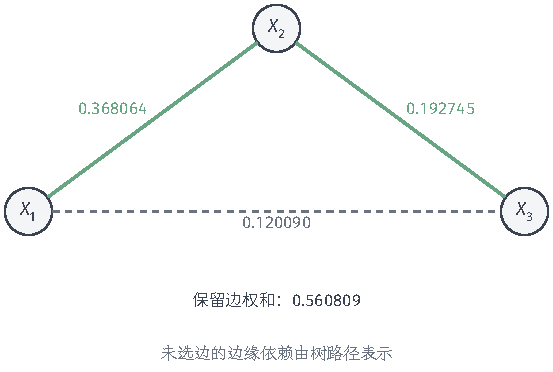
\includegraphics[width=\linewidth]{figures/03-models/03-probabilistic-graphical-models/tikz/pgm-structure-learning-chow-liu/figure.pdf}
  \caption{同一计数表产生的三个互信息边权，单位为nat。实线为最大权生成树保留的边，虚线为未选边。树分布在此例恰好复原经验分布，但算法一般只能给出最佳树近似。}
  \label{fig:pgm-structure-learning-chow-liu}
\end{figure}

选根为$1$时，所得模型取$p(X_1=1)=0.5$，沿两条边分别以$0.1$、$0.2$的概率翻转。于是$\widehat p_{\mathcal{T}}(0,0,0)=0.5\times0.9\times0.8=0.36$，与表中一致；每条记录平均对数似然为$-3\log2+0.368064+0.192745=-1.518633$，也复核了前面的BIC比较。

严格正边缘让证明免于处理零分母。若有零计数，可在经验支持上定义条件表，对从未出现的条件配置任取归一化版本，并采用$0\log0=0$延伸似然结论；若改用平滑伪计数，则优化的是平滑后的目标，不能仍声称是原记录的未惩罚最大似然估计。一般离散树的参数数目为
\[
  \sum_i(r_i-1)+
  \sum_{\{i,j\}\in E_{\mathcal{T}}}(r_i-1)(r_j-1).
\]
只有各节点状态数相同等情形下，所有树的维数才相同。即使状态数不同，Chow--Liu仍精确优化树族内似然，但若要作BIC选择，就应从每条互信息边权中扣除相应的参数惩罚。

树假设换来了高效的结构优化和推断，却排除了环及不可约高阶作用。即使总体图不是树，算法也会返回一棵树；“最优”只相对于候选树族。互信息接近时，有限样本可改变排序；零权边也可能仅为连接全部节点而被选入。允许森林并惩罚边数，可以不强迫所有变量相连。

\subsection{高斯图结构学习}
\label{sec:pgm-structure-learning-gaussian}

对非退化联合高斯变量，$\bm{X}\sim\mathcal{N}(\bm{\mu},\bm{\Sigma})$且$\bm{\Sigma}\succ0$，图结构可以直接从\term{精度矩阵}（precision matrix）$\bm{K}=\bm{\Sigma}^{-1}$读取：
\[
  X_i\perp X_j\mid\bm{X}_{V\setminus\{i,j\}}
  \quad\Longleftrightarrow\quad K_{i,j}=0.
\]
这与协方差零表示边缘独立不同。一般连续分布中，逆协方差的零元素也没有相同的条件独立保证。

令$\widehat{\bm{\Sigma}}=n^{-1}\sum_r(\bm{x}_r-\overline{\bm{x}})(\bm{x}_r-\overline{\bm{x}})^{\top}$。舍去常数并缩放后，高斯负对数似然为$-\log\det\bm{K}+\operatorname{tr}(\widehat{\bm{\Sigma}}\bm{K})$。直接求逆在$n$小于维数时可能不可行，在有限样本中也很少得到精确零。\term{图Lasso}（graphical lasso）加入稀疏惩罚：
\begin{equation}
  \widehat{\bm{K}}
  =\argmin_{\bm{K}\succ0}
    \left\{-\log\det\bm{K}
      +\operatorname{tr}(\widehat{\bm{\Sigma}}\bm{K})
      +\lambda\sum_{i\ne j}|K_{i,j}|\right\}.
  \label{eq:pgm-structure-learning-glasso}
\end{equation}
这里不惩罚对角元，惩罚同时计入两个对称非对角元素；与另一种仅对$i<j$求和的实现比较时应换算$\lambda$。正定约束保证合法高斯分布，$\ell_1$惩罚使部分非对角元恰好为零。该目标是凸的，但图恢复仍需要统计条件；一个可靠的凸求解器只能消除优化误差，不能消除抽样误差\scite{pgm-structure-learning-friedman2008}

也可逐节点估计邻域。高斯条件均值满足
\[
  \mathbb{E}[X_i\mid\bm{X}_{-i}]
  =\mu_i+\sum_{j\ne i}
    \left(-\frac{K_{i,j}}{K_{i,i}}\right)(X_j-\mu_j),
\]
其中$-i$表示除$i$外的所有节点。因此，对每个节点作稀疏线性回归，可以用非零回归系数估计邻居。两次回归对同一条边可能意见不同，取并集的OR规则偏向保留边，取交集的AND规则更保守。分别回归不自动给出对称正定的精度矩阵；若最终还要联合密度和推断，应另作相容参数拟合。

例如
\[
  \bm{K}=
  \begin{pmatrix}
    2&-1&0\\
    -1&2&-1\\
    0&-1&2
  \end{pmatrix},
  \qquad
  \bm{\Sigma}=\frac14
  \begin{pmatrix}
    3&2&1\\
    2&4&2\\
    1&2&3
  \end{pmatrix}.
\]
两矩阵相乘为单位矩阵，$\bm{K}$的顺序主子式为$2,3,4$，故正定。$\Sigma_{1,3}=1/4$虽非零，$K_{1,3}=0$却说明给定$X_2$以后两端独立。节点$1$的回归只保留$X_2$，系数为$1/2$；节点$2$对两端的系数均为$1/2$，恢复同一个无向链。实际选择$\lambda$时，预测误差最小的值不一定最利于精确选边，应区分预测调参与结构恢复目标。

\subsection{离散与高阶Markov网络结构学习}
\label{sec:pgm-structure-learning-discrete}

离散无向模型通常没有一个矩阵逆可以直接给出图。可先建立候选特征字典$\{f_a(\bm{x}_{C_a})\}$，其中$C_a\subseteq V$是特征作用域，再写成严格为正的有限状态模型
\[
  p_{\bm{\theta}}(\bm{x})
  =\exp\!\left\{\sum_a\theta_a f_a(\bm{x}_{C_a})
                    -A(\bm{\theta})\right\}.
\]
选哪些非零参数，就是选哪些相互作用；若每个候选作用域有一组编码参数，可以用组稀疏惩罚整体选择该因子。需要先规定可识别的编码或对比约束，否则同一分布的不同参数写法可能改变“哪些系数为零”。一个高阶因子还会把其作用域在无向图中补成团，因子集合比单纯边集保留了更细的建模信息。

完整似然加稀疏惩罚可写为
\[
  \min_{\bm{\theta}}\left\{
    A(\bm{\theta})-\sum_a\theta_a\widehat{\mathbb{E}}[f_a]
      +\lambda\lVert\bm{\theta}\rVert_1\right\}.
\]
计算梯度需要模型期望，也就需要推断；当候选作用域形成大团或大树宽时，这项代价会在每次优化中重复出现。另一条路线是\term{伪似然}（pseudolikelihood），以$\prod_{r,i}p_{\bm{\theta}}(x_{r,i}\mid\bm{x}_{r,-i})$代替联合似然。单点条件概率只需在$X_i$的状态上归一化，避开全局配分函数，但这不是原联合似然，也不自动继承其效率或有限样本性质。

例如对$x_i\in\{-1,1\}$的成对Ising模型，定义局部场$u_i=b_i+\sum_{j\ne i}J_{i,j}x_j$，则
\[
  \log\frac{p(X_i=1\mid\bm{x}_{-i})}
                {p(X_i=-1\mid\bm{x}_{-i})}=2u_i.
\]
节点邻域选择于是成为稀疏逻辑回归。若联合优化对称参数$J_{i,j}=J_{j,i}$，所得条件概率来自共同联合模型；若每个节点各拟合一组参数，还需处理两端选择和参数相容性。评分搜索也可直接增加、删除候选因子，但必须说明是在比较精确似然、近似似然还是伪似然。

只考察成对边缘可能完全漏掉高阶依赖。令
\[
  p(x_1,x_2,x_3)
  =\frac{\exp(\theta x_1x_2x_3)}{8\cosh\theta},
  \qquad x_i\in\{-1,1\},\quad \theta\ne0.
\]
对任一变量求和，分子变为$2\cosh\theta$，所以任意一对的边缘均为$1/4$，成对互信息全为零。但$\mathbb{E}[X_1X_2X_3]=\tanh\theta\ne0$，且给定$X_3$后$X_1,X_2$仍有相互作用。该分布严格为正，没有借助零概率事件；它需要三阶特征，不能由所有成对边缘的独立性得出联合独立。允许大小不超过$m$的作用域时，仅候选子集就有$\sum_{\ell=1}^{m}\binom d\ell$个，每个离散作用域内部还可能需要多个参数，搜索与样本需求都会增长。

\subsection{潜变量结构}
\label{sec:pgm-structure-learning-latent}

一张稠密的观测图可能来自许多直接相互作用，也可能只是若干共同未观测变量的结果。对联合高斯向量，把节点分成观测集合$O$和潜变量集合$H$，联合精度矩阵按这两个集合分块。对潜变量积分，或在二次型中配方，可得到观测边缘精度矩阵
\begin{equation}
  \begin{aligned}
    \bm{K}_{\mathrm{marg}}
      &=(\bm{\Sigma}_{O,O})^{-1}\\
      &=\bm{K}_{O,O}
        -\bm{K}_{O,H}\bm{K}_{H,H}^{-1}\bm{K}_{H,O}\\
      &=\bm{S}-\bm{L}.
  \end{aligned}
  \label{eq:pgm-structure-learning-schur}
\end{equation}
$\bm{S}=\bm{K}_{O,O}$是给定潜变量后的条件精度矩阵，而$\bm{L}\succeq0$且$\operatorname{rank}(\bm{L})\leq|H|$。若条件图稀疏、有效潜变量少，便得到常称的\term{稀疏加低秩分解}（sparse plus low-rank decomposition）；按这里的半正定约定，公式实际上是稀疏项减低秩项。

一个可复核的例子是$X_i=Z+\varepsilon_i$，$i=1,2,3$，其中$Z,\varepsilon_1,\varepsilon_2,\varepsilon_3$为相互独立的标准高斯变量。给定$Z$后三个$X_i$独立，但边缘协方差为$\bm{I}+\bm{1}\bm{1}^{\top}$，由直接相乘可验证
\[
  \bm{K}_{\mathrm{marg}}
  =\bm{I}-\frac14\bm{1}\bm{1}^{\top}.
\]
非对角元全为$-1/4$，所以只看观测量得到完整条件依赖图；这里$\bm{S}=\bm{I}$，$\bm{L}=\bm{1}\bm{1}^{\top}/4$的秩为1。稠密观测依赖和给定潜变量后的独立并不矛盾。

令$\widehat{\bm{\Sigma}}_{O,O}$为观测样本协方差，可以求解
\begin{equation}
  \begin{aligned}
    \min_{\bm{S},\bm{L}}\quad&
      -\log\det(\bm{S}-\bm{L})
      +\operatorname{tr}\!\left(
           \widehat{\bm{\Sigma}}_{O,O}(\bm{S}-\bm{L})\right)\\
      &+\lambda\bigl(\gamma\lVert\bm{S}\rVert_1
                      +\operatorname{tr}(\bm{L})\bigr),\\
    \text{满足}\quad&\bm{S}-\bm{L}\succ0,\qquad \bm{L}\succeq0.
  \end{aligned}
  \label{eq:pgm-structure-learning-sparse-low-rank}
\end{equation}
此处$\lVert\bm{S}\rVert_1$为逐元素绝对值之和，包含对角项；$\gamma>0$调节两种惩罚的相对强度。半正定矩阵的核范数等于迹，因此第二个惩罚鼓励低秩。该凸程序的可识别性与恢复理论要求稀疏结构和低秩结构足够可区分，例如潜变量影响应分散到较多观测节点，不能本身又集中成很稀疏的模式\scite{pgm-structure-learning-chandrasekaran2012}

即使精确知道$\bm{K}_{\mathrm{marg}}$，分解也不总唯一：既稀疏又低秩的分量可以在两项之间移动而保持差不变。可识别条件满足时，$\bm{L}$的秩刻画有效潜在维数；它不自动等于全部物理隐因数量，潜变量的旋转、重参数化和具体含义还可能无法确定。完整潜变量图、给定潜变量后的观测条件图$\bm{S}$，以及边缘化后的观测图$\bm{K}_{\mathrm{marg}}$是三个不同对象。此处的低秩表示是一种统计分解，不是潜在因果图已被恢复的证明。

\section{因果发现}
\label{sec:pgm-structure-learning-causal}

前面的目标是表示分布。若还要判断改变一个变量会不会影响另一个变量，就必须给图增加干预含义。不同发现方法所用的信息不相同，其输出应与能成立的识别结论绑定，而不是一律画成“真实因果网络”。

\subsection{因果假设与识别目标}
\label{sec:pgm-structure-learning-causal-assumptions}

\term{因果Markov性}（causal Markov condition）要求观测分布相对于因果有向图满足Markov性质；前面引入的忠实性进一步排除不由d-分离解释的额外独立性。前者允许沿图从机制推出独立性，后者允许从独立性反推图约束。例如两条因果路径的效应恰好抵消时，Markov性仍可能成立，忠实性却失败。有限样本还会遇到近似抵消，检验可能难以区分极弱联系和零联系。

\term{因果充分性}（causal sufficiency）要求相对于当前节点集合的共同直接原因都已被观测，也就是没有未建模的潜在混杂。它不要求世界上所有变量都已被测量。通常还要假定因果过程无环、样本没有未建模的选择偏差，以及数据来自所声明的环境。若要借助函数形式突破等价类，还需线性、噪声独立、非高斯性等对应条件。这些假设不是换一个搜索器就能自动获得的。

在充分、无环且忠实的观测设置下，条件独立信息一般只识别CPDAG。若允许潜变量，就需要把完整有向图边缘化后的关系表示出来。\term{最大祖先图}（maximal ancestral graph, MAG）用有向边、双向边及在考虑选择偏差时的无向边，表示观测变量的条件独立关系，而不显式画出所有潜变量。它无有向环；若一条边在$i$端有箭头，$i$不能是另一端的祖先；与无向边相接的节点不能再有任何箭头指入。其“最大”指任何不相邻点对都可被某组观测变量分离，不是边越多越好。混合图中的\term{m-分离}（m-separation）按两侧箭头识别路径上的碰撞节点：路径活跃要求每个非碰撞节点不在条件集合中，每个碰撞节点自身或至少一个后代在条件集合中。不存在连接两端的活跃路径，才称被m-分离。

\term{部分祖先图}（partial ancestral graph, PAG）表示一组Markov等价MAG的共同端点信息。尾端和箭头端表示类内不变的端点，圆圈表示该端点在类内尚不确定；圆圈不是“可能没有边”。在不考虑选择偏差时，$i\to j$表达祖先关系，未必是观测尺度下的一条直接因果机制；$i\leftrightarrow j$排除二者互为祖先，并与潜在混杂相容，不表示双向反馈；$i\mathbin{\circ\!\!\to}j$只固定$j$端的箭头，不能把$i$端圆圈偷偷补成尾端。PAG编码祖先关系和独立性层面的不确定性，不枚举潜变量个数和连线细节\scite{pgm-structure-learning-zhang2008}

\subsection{基于观测数据的因果发现}
\label{sec:pgm-structure-learning-observational}

第~\ref{sec:pgm-structure-learning-directed}节已经说明了PC和GES如何使用检验或评分。它们在因果发现中的额外问题是：统计等价类能否解释为因果等价类。PC在因果Markov性、忠实性、因果充分性、无环性及正确独立性判定下返回CPDAG；有限样本检验只能给出该对象的估计。GES也不凭评分消除观测等价：当评分等价、可分解且局部一致，真实分布忠实于候选族中的有向图，并满足相应固定维大样本条件时，其等价类搜索可恢复CPDAG。这里的局部一致性是指，大样本时评分奖励加入当前模型确实遗漏的依赖，并惩罚多余依赖，不只是笼统地说“评分一致”。

允许潜在混杂时，PC使用的邻域分离搜索不再有相同保证。\term{快速因果推断算法}（fast causal inference, FCI）扩展需要考察的分离集合，并使用祖先图的定向规则，在相应Markov性、忠实性和准确条件独立信息下输出PAG。它可以容纳潜变量，标准框架也能处理所声明的选择机制，但并不因此免除其他假设。即使有无限观测数据，FCI通常也不输出唯一完整因果有向图；把PAG中所有圆圈强制定向，会丢掉算法本来保留的不确定性。完整定向规则及其识别边界见Zhang的研究\scite{pgm-structure-learning-zhang2008-completeness}

另一种方向信息来自分布形状，而不只是条件独立。\term{线性非高斯无环模型}（linear non-Gaussian acyclic model, LiNGAM）设
\[
  X_j=\sum_{i\in\operatorname{pa}(j)}b_{j,i}X_i+\varepsilon_j,
\]
其中图无环，扰动相互独立、方差有限且非零、分布非高斯，不存在未观测混杂。令$\bm{B}$的第$(j,i)$个元素为$b_{j,i}$，$\bm{\varepsilon}$为扰动向量，递归展开得到$\bm{X}=(\bm{I}-\bm{B})^{-1}\bm{\varepsilon}$。\term{独立成分分析}（independent component analysis, ICA）从混合观测中分离统计独立的源；在这里可以利用非高斯性区分扰动，再结合无环结构约束消除相关排列歧义，从而在模型条件下识别超出MEC的方向。线性高斯模型没有同样的信息，所以不能省去“非高斯”二字后仍保留结论\scite{pgm-structure-learning-shimizu2006}

\term{加性噪声模型}（additive noise model, ANM）允许$Y=f(X)+\varepsilon$且$\varepsilon\perp X$。在适当的光滑性、非退化及可识别性条件下，正向能表示为独立加性噪声，并不意味着反向也能表示为$X=g(Y)+\eta$且$\eta\perp Y$。比较拟合残差与输入的独立性便可提供方向证据；这与仅比较回归误差不同。多变量版本还要求递归机制和相互独立的扰动。线性高斯等例外在两个方向上都可成立，不能声称所有非线性回归都能恢复真因果\scite{pgm-structure-learning-peters2014}

\subsection{基于干预数据的因果发现}
\label{sec:pgm-structure-learning-interventional}

对表~\ref{tab:pgm-structure-learning-counts}，观测$X_2=1$时，$X_1$取$1$的频率为$0.9$。这不能直接回答把$X_2$外部设置为$1$后，$X_1$是否也会改变。若真实机制是$X_1\to X_2\to X_3$，设置中间节点不会反向改变$X_1$；若机制是分叉$X_1\leftarrow X_2\to X_3$，则会影响$X_1$。干预通过改变数据产生过程，而不是多收集同一种观测，区分了这两种解释。

\term{完美干预}（perfect intervention）替换目标节点的原机制，使其不再依赖原父节点，并保持非目标节点机制不变。设已知目标集合$I\subseteq V$，对目标独立随机化，赋予外部规定的分布$q_i^I$，则
\begin{equation}
  p^I(\bm{x})
  =\prod_{i\in I}q_i^I(x_i)
   \prod_{j\notin I}
      p(x_j\mid\bm{x}_{\operatorname{pa}_{\mathcal{G}}(j)}).
  \label{eq:pgm-structure-learning-intervention}
\end{equation}
图上这对应删除所有进入$I$的箭头，记干预图为$\mathcal{G}^{[I]}$；空目标$I=\varnothing$对应观测环境。固定某个取值的干预可作退化版本，但用条件独立刻画等价类时，通常使用具有足够支持的随机化干预或覆盖所需取值的实验，避免固定变量造成退化。

设$\mathcal{I}$是已知干预目标集合组成的族。它是\term{保守的}（conservative），若每个节点都至少在一个环境中未被干预；只要包含观测环境就满足这一条件。\term{干预Markov等价类}（interventional Markov equivalence class, I-MEC）是在给定$\mathcal{I}$及完美干预约定下，允许相同多环境分布族的有向图集合。这里多环境分布要求共享非目标机制，不是任意独立挑选各环境的分布。

在保守目标族及相应正性设定下，两个有向图干预等价，当且仅当它们观测Markov等价，且对每个$I\in\mathcal{I}$，删去目标入边后的两个干预图有相同骨架。等价地，也可要求观测图的骨架与v-结构相同，并比较各干预图的Markov等价关系。\term{干预本质图}（interventional essential graph）把I-MEC中所有有向图共同的方向画为有向边，其余画为无向边。I-MEC细分观测MEC，但目标选择不充分时仍可能含多张图\scite{pgm-structure-learning-hauser2012}

沿用二值例子，给三种观测等价图分别配置能够复原同一张表的局部条件分布。在$\operatorname{do}(X_2=1)$下，正向链预测$(p(X_1=1),p(X_3=1))=(0.5,0.8)$，分叉预测$(0.9,0.8)$，反向链预测$(0.9,0.5)$。三个答案不同，而在观测条件$X_2=1$下它们都给出$(0.9,0.8)$。图~\ref{fig:pgm-structure-learning-intervention}显示，在观测环境之外，对$X_2$进行覆盖两种取值的完美干预可以区分这三种结构；这是总体层面的识别，不是有限样本下看到一个频率差就必然定向正确。

\begin{figure}[htbp]
  \centering
  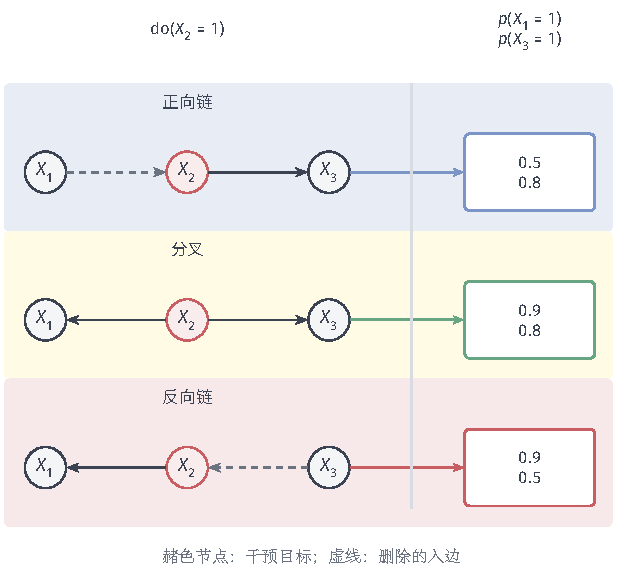
\includegraphics[width=\linewidth]{figures/03-models/03-probabilistic-graphical-models/tikz/pgm-structure-learning-intervention/figure.pdf}
  \caption{同一观测MEC在干预$X_2$后产生不同预测。蓝、黄、红三条横带分别对应正向链、分叉和反向链，右侧概率框用同色箭头与结构逐行映射；实线为干预后的保留边，虚线为被切断的入边。在该三节点例子及给定假设下，这些预测足以区分三个方向。}
  \label{fig:pgm-structure-learning-intervention}
\end{figure}

\term{贪心干预等价搜索}（greedy interventional equivalence search, GIES）在干预本质图空间中搜索，结合前向、后向以及转向操作比较I-MEC。每条样本必须带有目标标签$I_r$。若目标随机化分布已知或不依赖候选图，去掉相同常数后的机制对数似然为
\[
  \ell(\mathcal{G},\bm{\theta})
  =\sum_{r=1}^{n}\sum_{j\notin I_r}
       \log p_{\bm{\theta}_j}
          (x_{r,j}\mid\bm{x}_{r,\operatorname{pa}(j)}).
\]
被干预节点的记录不用于拟合该节点的原机制，但仍可用于其子节点的机制拟合。适用于干预数据的惩罚评分还需考虑各机制可用的样本量，不能把不同环境全部当作同分布观测直接套普通评分。GIES利用这些得分在I-MEC之间移动，目标是联合利用观测与干预信息；其名称本身不提供无条件的全局最优或因果恢复保证。

若干预目标未知，环境标签只表明机制发生了某种改变，还需联合推断目标，并限定哪些机制可变、变化是否足够可检测、非目标机制是否保持不变；若是软干预，只改变部分机制参数而不切断全部父依赖，上述删边图与I-MEC定义就不再原样适用。干预不完全、执行不依从、同时影响多个未知节点，或者非目标机制随环境漂移，也会改变识别条件。即使目标已知，未经建模的潜在混杂仍会使普通充分有向图版本的GIES不适用。

\term{主动实验设计}（active experimental design）是在预算允许的目标中，选择预计最能区分当前候选结构的下一次干预。例如三节点链中，重复被动观测不能决定可逆方向，而干预中间节点可使三个候选给出不同预测。具体设计可按预期后验熵下降、待定端点减少或目标科学问题的区分度来选择，并把成本和可执行性加入约束。计划中的“信息增益”仍基于当前模型及机制不变假设，不应把它当作尚未实施实验的结果。

表~\ref{tab:pgm-structure-learning-causal-routes}归纳各路线的假设与输出。它不是互斥的算法分类：ANM可同时使用回归、独立性检验和评分，连续优化也可求解带特定函数假设的目标。决定识别能力的是模型与数据提供了什么信息，而不是代码是否使用梯度。

\begin{table*}[htbp]
  \centering
  \small
  \begin{tabularx}{\linewidth}{@{}lXX@{}}
    \toprule
    路线 & 关键条件与信息 & 理想识别对象及限制 \\
    \midrule
    PC & 无环、因果充分、Markov且忠实；准确独立性信息 & CPDAG；不决定类内可逆方向 \\
    GES & 相应充分有向图模型；评分等价、可分解、局部一致 & 大样本下CPDAG；不是一般贪心搜索的保证 \\
    FCI & 允许潜在混杂；相应Markov性、忠实性及选择机制假设 & PAG；不是潜变量完整图 \\
    LiNGAM & 线性无环、独立非高斯扰动、无潜在混杂 & 模型条件下单个有向图；依赖分布形状 \\
    ANM & 独立加性噪声、无混杂及特定可识别性条件 & 满足条件时单个有向图；存在双向可表示例外 \\
    GIES & 已知目标的完美干预、无混杂、机制不变、相应评分 & 搜索I-MEC；并非一般全局最优保证 \\
    \bottomrule
  \end{tabularx}
  \caption{识别假设决定可追求的输出。表中的理想对象以总体条件成立为前提，实际算法还受有限样本、模型拟合和搜索误差影响。}
  \label{tab:pgm-structure-learning-causal-routes}
\end{table*}

\subsection{因果发现的边界}
\label{sec:pgm-structure-learning-causal-limits}

结构不确定性至少有三种不同来源。有限样本误差使检验和评分偏离总体结论，更多同类数据有机会减少它；模型假设错误，例如存在潜在混杂却使用因果充分算法，可能让更多数据更稳定地支持错误解释；总体不可识别则意味着多个结构对所有允许的数据都给出同样的分布，单纯增大样本量不能区分。诊断结果时，应明确当前顾虑属于哪一类，才能决定补样本、改模型还是增加实验信息。

观测等价不是算法实现不够好，PAG中的圆圈也不是必须消灭的绘图缺陷。领域知识可以排除部分结构，但这些方向应标记为先验约束的贡献；函数形式能够增加可识别性，但必须接受检验这些形式假设的责任。没有独立依据时，一张稀疏、有向且重复出现的图，仍不足以证明其为真实因果结构。

本节只回答结构发现的目标及识别边界。某个干预效应是否可由现有数据计算，是因果效应识别的问题；do演算及反事实推断还有各自的定义和条件。恢复部分结构并不等于已解决所有效应查询，不能把这里的结构结果直接当作任意政策或个体反事实结论。

\section{算法分析}
\label{sec:pgm-structure-learning-analysis}

把数据、假设、评分和搜索区分以后，才有可能准确评价一个结构学习结果。“一致”“最优”“稳定”分别回答不同问题，彼此不能替代。

\subsection{统计一致性与有限样本误差}
\label{sec:pgm-structure-learning-consistency}

设$\mathcal{C}^{*}$表示在声明的信息下可识别的目标，例如一个CPDAG而不是任意真实有向图。\term{结构一致性}（structural consistency）通常要求$\mathbb{P}(\widehat{\mathcal{C}}_n=\mathcal{C}^{*})\to1$。目标写成什么，结论就只能达到哪里。树分布不成立时，Chow--Liu可趋向最佳树近似；这不等于恢复生成分布的真实图。图Lasso的参数误差趋零也不自动意味着零元素模式完全正确，还需要非零边与零之间具有足够间隔。

PC的一致性取决于会执行的条件独立判断能同时趋于正确，而不是每个检验看起来有合理的$p$值。若需考虑的检验集合大小为$M$，并且每项错误概率都至多为$\delta$，则联合界给出至少一次错误的概率不超过$M\delta$，不要求检验独立。对自适应选取的检验，必须控制全部可能被选中的相关集合，不能只事后数实际执行了多少次。固定显著性水平一般也不足以保证整体选图错误概率随$n$消失，需要相应阈值序列和功效条件。

弱边是统计困难的直接来源。高斯检验中，非零偏相关若小于估计波动尺度，就难以可靠保留；离散检验中，条件集扩大使每个配置可用的样本减少。高维稀疏性可以限制必要条件集大小，但仍需控制最大度、变量状态数、协方差条件数或最小信号等量，不能仅以“图稀疏”概括全部一致性假设。

BIC的一致性解释也有条件。在固定维、正确设定及常规正则条件下，遗漏真实依赖通常造成随$n$线性增长的似然损失，而不必要的参数所获得的随机拟合收益通常仅为有界概率量级，$\log n$惩罚因而有机会区分二者。该论证针对候选模型比较；搜索器若没有到达正确模型，评分的一致性不会自动挽救搜索结果。潜变量奇异性或维数随样本增长时，不能直接照搬这一理由。

Chow--Liu的有限样本稳定性可以用一个更具体的间隔解释。设$d\geq3$且总体最大权生成树唯一，对每条不在树中的边$e$，考察其连接路径上的各树边$f$，定义
\[
  \Delta=\min_{e\notin E_{\mathcal{T}^{*}}}
             \min_{f\in\operatorname{path}_{\mathcal{T}^{*}}(e)}
             \{I_f-I_e\}.
\]
当$\Delta>0$，且所有经验互信息误差都小于$\Delta/2$时，各非树边与路径边的关键次序保持不变，最大权生成树不变。三节点例子中这个间隔约为$0.072654$，由两条较小互信息之差得到。若间隔为零，树结构可能不唯一，即使分布预测相近，具体边的选择也可能随样本扰动改变。

\subsection{计算复杂度与可扩展性}
\label{sec:pgm-structure-learning-complexity}

不同算法的主要成本并不相同。PC的成本由条件集枚举和每次检验决定；若整个搜索过程中候选邻域大小被$q$控制，一个粗略检验数上界为$O(d^2 2^q)$，再乘单次检验代价。这个$q$不是无条件等于真实最大度：有限样本误保留的边也可能扩大邻域。FCI需搜索更丰富的分离集合，通常比同规模PC承担更多工作。

完整离散有向图的局部评分可缓存，但每个节点仍可能有指数多候选父集。动态规划在预计算好最佳父集表后，常见的子集递推为$O(d2^d)$时间量级，局部表的准备与存储本身也很昂贵；整数规划的分支搜索同样可能指数增长。局部有向图搜索单轮可以考察$O(d^2)$个边操作，但轮数、无环检查和局部拟合代价仍需另外计算，不能把单轮操作数当作总复杂度。

若各离散变量状态数有界，Chow--Liu可用$O(nd^2)$时间累积成对计数，再在稠密完全图上用$O(d^2)$时间量级的Prim算法求树，或排序边后用$O(d^2\log d)$的Kruskal算法。完成模型后，树上的一次有限状态边缘推断随节点数线性增长。它同时简化学习与推断，但这个优势以树族的表达限制为代价。

稠密NOTEARS实现中，计算$\bm{Y}\bm{W}$约需$O(nd^2)$运算，矩阵指数通常涉及$O(d^3)$量级的稠密线性代数；还要乘以内部优化和惩罚更新的轮数。图Lasso也有矩阵更新成本，但其目标凸；稀疏邻域回归容易按节点并行，却需处理估计的一致性。高阶离散模型的瓶颈可能不是枚举边，而是在每次评分时计算配分函数。最大父集、候选筛选和限制作用域等手段，应同时报告它们节省了什么计算、排除了哪些结构。

\subsection{结构评价与稳定性}
\label{sec:pgm-structure-learning-evaluation}

有已知生成图的仿真中，可以分别评价骨架和方向。骨架精确率为正确预测边数除以预测边数，召回率为正确预测边数除以真实边数；分母为零时应预先规定记法。方向评价应明确是只在骨架预测正确的边上计算，还是把漏边也纳入分母。若真实可识别对象只是CPDAG，就不应把算法没有猜中某个代表有向图的可逆方向算作错误，也不应因算法任意猜对该方向就奖励其识别能力。

\term{结构Hamming距离}（structural Hamming distance, SHD）统计把估计图变为目标图所需的边编辑数。常用有向图约定把一次加边、删边或反向各计1；有些实现把反向计为一次删除加一次添加，因此比较结果必须注明口径。对CPDAG，应先把真有向图转为相应等价类表示，再分别比较邻接、被迫方向和未定向状态；对PAG，还需评价圆圈、尾端和箭头端，不能直接套二值邻接矩阵的距离。

真实数据中往往没有真图可比。\term{自助重采样}（bootstrap）可以从$n$条独立记录中有放回抽取$n$条，重复拟合$B$次，并记录某条边的出现频率
\[
  \widehat\pi_{i,j}
  =\frac1B\sum_{b=1}^{B}
       \mathbf{1}\{\{i,j\}\text{在第}b\text{次结果中相邻}\}.
\]
方向频率应另行统计，并声明分母是所有重复，还是只包括该边出现的重复。CPDAG中未定向的结果不能被强制补全后计成方向支持；每轮的调参和筛选是否重做，也会影响稳定性含义。多环境数据应在环境内重采样，相关序列则需适当的块重采样，不能把不独立的记录当作独立单位。

重采样频率衡量流程对数据扰动的敏感性，不是结构后验概率，也不是因果真实性概率。一个错误的先验限制或错误的分布假设可能在每轮都产生同一个错误结果。还应比较不同正则强度、独立性检验设置和合理模型假设下的变化，并用独立验证数据评价预测表现；预测好本身仍不能证明方向正确。

领域知识可以直接进入候选空间。禁止边使其候选局部得分不可用，必选边限制允许父集，时间顺序排除逆时间箭头；进入搜索前还要检查这些约束是否彼此矛盾或已经形成有向环。在等价类输出中，应区分数据确定的方向和背景知识补充的方向，并相对于加入相同知识后的识别对象评价。这样报告的结构才同时说明“看到了什么”和“事先假定了什么”。

\section{本章小结}
\label{sec:pgm-structure-learning-summary}

从记录中学习图，不是把相关系数变成连线这么简单。条件独立约束回答哪些联系可以被给定变量隔断，评分衡量候选分布的拟合和复杂度，搜索决定怎样遍历合法结构。三者可以组合，却承担不同责任。Chow--Liu之所以能够精确求解，是因为树的最佳似然分解为互信息边权之和；一般有向图和高阶无向模型没有同样的简化。

结构输出必须与信息相称。同一张计数表可以支持一个无向链、一个有向图等价类，也可以给多个图赋予后验权重，但不能仅凭观测频率决定链的因果方向。缺失数据需要推断未观测统计量，潜变量可能把稀疏条件图变成稠密边缘图；这些变化不仅增加计算量，也改变可识别的对象。因果发现只有在明确的机制、混杂、忠实性或函数形式假设下，才可把统计证据解释为CPDAG、PAG或更细的干预等价类。

因此，一个可信的结构学习结论应同时给出候选模型、数据和干预条件、评分或检验、搜索限制，以及输出中的不确定性。样本更多、优化更充分和模型假设更合适，分别解决不同问题；观测层面的不可识别仍可能需要新的实验信息。回到章首，数据能够帮助选择解释依赖的图，但箭头是否代表故障传播，必须由相应的识别假设和干预证据承担，而不能由绘图代替论证。

后续模型章节将改变提问方式：给定分类、潜在分组或状态估计任务，哪些结构假设能同时满足表达与计算需要？第~\ref{chap:pgm-static-directed}章从静态有向模型开始，把前面的分解、推断和学习方法用于具体模型。采用一种模型结构，仍不等于其潜变量已获得唯一的物理解释。
